\section{Task 2: Baseline Model Construction and 2D Segmentation Training}

The goal of this task is to build a complete baseline pipeline for 2D brain tumor segmentation. The task requires a basic encoder--decoder network, a loss function suitable for severe foreground-background imbalance, data augmentation, 2D slice-based training from 3D MRI volumes, and preliminary evaluation using Dice scores. This report is self-contained: all key dataset definitions, label meanings, model settings, experimental comparisons, loss-curve interpretations, visualization summaries, and conclusions are described here.

The final selected baseline is a 2D U-Net trained with three MRI modalities as input: \texttt{t2f}, \texttt{t1c}, and \texttt{t2w}. The model predicts the original four-class segmentation labels. Several additional models were trained to answer two design questions: first, which modality combination is most useful; second, whether predicting original multiclass labels or derived clinical regions is better for this baseline.

\subsection{Dataset and Preprocessing}

Each 2D training sample contains four aligned MRI modalities with spatial size \(177 \times 219\). The four modalities are \texttt{t1n}, \texttt{t1c}, \texttt{t2w}, and \texttt{t2f}. The segmentation target uses the original label definition shown in Table~\ref{tab:labeldef}.

\begin{table}[h]
\centering
\begin{tabular}{cl}
\hline
Label & Meaning \\
\hline
0 & Background \\
1 & NCR/NET, necrotic and non-enhancing tumor core \\
2 & ED, peritumoral edema \\
3 & ET, enhancing tumor \\
\hline
\end{tabular}
\caption{Original multiclass label definition. These label meanings are fixed throughout the report.}
\label{tab:labeldef}
\end{table}

The preprocessing pipeline has four main steps. First, non-informative empty space around the brain is cropped so that the model focuses on useful image content. Second, Z-score normalization is performed separately for each patient and each modality over non-background voxels. This is necessary because MRI intensity values are not standardized across patients. Third, background voxels are set to zero after normalization. Fourth, the preprocessed 3D volumes are sliced into 2D axial images.

Fully black slices are removed before training and evaluation. These slices contain no useful anatomical or tumor information, so including them would waste training iterations and encourage a trivial background prediction. The split is performed at the patient level instead of the slice level to avoid data leakage between adjacent slices from the same patient. The final split ratio is \(70\%:10\%:20\%\) for training, validation, and testing. This gives 437 training patients, 62 validation patients, and 126 test patients, corresponding to 67,735 training slices, 9,610 validation slices, and 19,530 test slices.

\subsection{Derived Clinical Regions}

The original labels in Table~\ref{tab:labeldef} are not changed. For evaluation, they are combined into three derived clinical regions:

\[
WT=\{1,2,3\}, \qquad TC=\{1,3\}, \qquad ET=\{3\}.
\]

WT means whole tumor and includes NCR/NET, ED, and ET. TC means tumor core and includes NCR/NET and ET, but not ED. ET corresponds exactly to original label 3. Therefore:

\[
WT = NCR/NET + ED + ET, \qquad
TC = NCR/NET + ET, \qquad
ET = ET.
\]

This distinction is important. Label 1 is always NCR/NET, label 2 is always ED, and label 3 is always ET. WT and TC are not new original labels; they are region combinations derived from the original annotation.

\subsection{Why Different Modality Combinations Were Tested}

Brain tumor MRI segmentation is naturally multimodal. Different MRI sequences emphasize different tissue properties, so no single modality fully captures every tumor component. A useful baseline should therefore test whether complementary modalities improve segmentation compared with single-modality inputs.

\texttt{t1n} mainly provides anatomical structure, but it has weak tumor-background contrast. It is still useful as a low-information baseline. \texttt{t1c} is contrast-enhanced T1 imaging and is expected to be more useful for enhancing tumor and tumor core. \texttt{t2w} and \texttt{t2f} are more sensitive to fluid-related abnormalities, so they are important for edema and whole-tumor extent.

The normalized contrast values used to guide modality selection are shown in Table~\ref{tab:contrast}. Higher values indicate stronger tumor-background separation.

\begin{table}[h]
\centering
\begin{tabular}{lccc}
\hline
Modality & WT & TC & ET \\
\hline
\texttt{t1n} & -0.037 & -0.212 & -0.100 \\
\texttt{t1c} & 0.311 & 1.396 & 2.078 \\
\texttt{t2w} & 0.957 & 1.180 & 0.931 \\
\texttt{t2f} & 2.659 & 2.867 & 2.847 \\
\hline
\end{tabular}
\caption{Mean normalized contrast by modality and derived clinical region.}
\label{tab:contrast}
\end{table}

The modality experiments were designed in a sequence. The \texttt{t1n}-only model tests a weak anatomical baseline. The \texttt{t1c}-only model tests a stronger enhancement-sensitive baseline. The selected multimodal model tests whether \texttt{t2f}, \texttt{t1c}, and \texttt{t2w} provide complementary information. The all-modality model tests whether adding every available modality is automatically better.

\subsection{Why Multiclass and Region Targets Were Both Tested}

The original annotation can be used in two training formats. In the multiclass formulation, the model predicts one four-class label map:

\[
0=\mathrm{background}, \quad
1=\mathrm{NCR/NET}, \quad
2=\mathrm{ED}, \quad
3=\mathrm{ET}.
\]

This formulation is mutually exclusive: each pixel belongs to exactly one class. It directly matches the original labels and works naturally with Cross Entropy Loss.

In the region formulation, the original labels are converted into three binary maps: WT, TC, and ET. This is clinically meaningful because these are the final evaluation regions. However, the region maps are nested:

\[
ET \subseteq TC \subseteq WT.
\]

If the three binary maps are predicted independently, this nesting relationship is not automatically guaranteed. Therefore, the comparison tests an important trade-off: direct optimization of clinical regions versus the structural simplicity of original multiclass prediction.

\subsection{Network Architecture}

The model is a plain 2D U-Net. The selected input has shape:

\[
[B,3,177,219],
\]

where the three channels are \texttt{t2f}, \texttt{t1c}, and \texttt{t2w}. For multiclass segmentation, the output has shape:

\[
[B,4,177,219].
\]

The encoder consists of convolution blocks followed by max pooling. Each convolution block contains two \(3 \times 3\) convolutions, batch normalization, ReLU activation, and dropout. The decoder upsamples feature maps and concatenates them with encoder features through skip connections. The final \(1 \times 1\) convolution maps the decoder features to segmentation logits.

The final architecture uses 3 input channels, 4 output channels, base channel width 32, encoder widths 32, 64, 128, and 256, bottleneck width 512, and dropout 0.1. This architecture is intentionally simple because Task 2 focuses on constructing a reliable baseline rather than introducing complex fusion modules.

\subsection{Loss Function Design}

Medical image segmentation has severe class imbalance. Most pixels belong to background, while tumor subregions, especially ET, occupy much smaller areas. To address this imbalance, the final multiclass model uses a hybrid loss:

\[
\mathcal{L}_{total} =
\mathcal{L}_{CE} + \mathcal{L}_{Dice}.
\]

Cross Entropy Loss provides stable pixel-wise multiclass supervision. Dice Loss directly optimizes overlap and is less dominated by background pixels. For class \(c\), the Dice score is:

\[
Dice_c =
\frac{2\sum_i p_{i,c}g_{i,c}+\epsilon}
{\sum_i p_{i,c}+\sum_i g_{i,c}+\epsilon},
\]

where \(p_{i,c}\) is the predicted probability and \(g_{i,c}\) is the one-hot ground truth. The Dice loss is:

\[
\mathcal{L}_{Dice}=1-\frac{1}{C}\sum_{c=1}^{C}Dice_c.
\]

The final setting uses equal weights for Cross Entropy and Dice Loss, with smoothing value \(10^{-5}\).

\subsection{Data Augmentation}

The training pipeline applies random rotation, horizontal flipping, vertical flipping, random scaling, and Gaussian noise. The final settings are:

\begin{itemize}
    \item rotation range: \([-15^\circ,15^\circ]\);
    \item horizontal flip probability: 0.5;
    \item vertical flip probability: 0.5;
    \item scaling range: \([0.9,1.1]\);
    \item Gaussian noise probability: 0.3;
    \item Gaussian noise standard deviation: 0.05;
    \item padding before spatial transforms: 24 pixels.
\end{itemize}

The same spatial transform is applied to the image and mask. The image uses bilinear interpolation, while the mask uses nearest-neighbor interpolation to preserve discrete label values. Gaussian noise is added only to the image.

\subsection{Training Strategy}

The model is trained on 2D slices rather than full 3D volumes to reduce memory cost and provide a straightforward baseline. The final training configuration uses batch size 8, maximum 100 epochs, AdamW optimizer, initial learning rate \(3 \times 10^{-4}\), weight decay \(1 \times 10^{-4}\), automatic mixed precision, gradient clipping norm 1.0, and random seed 42.

The learning rate is controlled by ReduceLROnPlateau. The scheduler monitors validation loss, uses factor 0.5, patience 10, threshold \(10^{-4}\), and minimum learning rate \(10^{-6}\). This schedule is useful because segmentation training often improves quickly at first and then requires a smaller learning rate to refine boundaries and small tumor regions.

\subsection{Preliminary Evaluation Metrics}

The main evaluation metric is Dice coefficient for WT, TC, and ET:

\[
Dice = \frac{2|P \cap G|}{|P|+|G|},
\]

where \(P\) is the predicted region and \(G\) is the ground truth region. The mean Dice is the average of WT, TC, and ET Dice scores.

For the final selected model, the best validation mean Dice occurs at epoch 33, as shown in Table~\ref{tab:bestval}.

\begin{table}[h]
\centering
\begin{tabular}{ccccccc}
\hline
Epoch & Train loss & Val loss & WT & TC & ET & Mean \\
\hline
33 & 0.1168 & 0.3646 & 0.9369 & 0.9454 & 0.8985 & 0.9269 \\
\hline
\end{tabular}
\caption{Best validation Dice of the final selected model.}
\label{tab:bestval}
\end{table}

The final test result of the selected model is shown in Table~\ref{tab:finaltest}.

\begin{table}[h]
\centering
\begin{tabular}{lccccc}
\hline
Model & Test loss & WT & TC & ET & Mean \\
\hline
Selected multimodal multiclass & 0.2224 & 0.9369 & 0.9519 & 0.8997 & 0.9295 \\
\hline
\end{tabular}
\caption{Test performance of the final selected baseline.}
\label{tab:finaltest}
\end{table}

\subsection{Experiment Comparison Overview}

The completed experiments are summarized in Table~\ref{tab:allresults}. The table gives the overall numerical comparison, while the following subsections discuss each model separately. Each model subsection includes the purpose, quantitative result, and a self-contained loss-curve and visualization summary.

\begin{table}[h]
\centering
\begin{tabular}{llccccc}
\hline
Model & Target & Modalities & Loss & WT & TC & ET & Mean \\
\hline
\texttt{t1n}-only & multiclass & \texttt{t1n} & 0.4856 & 0.7637 & 0.6485 & 0.4954 & 0.6359 \\
\texttt{t1c}-only & multiclass & \texttt{t1c} & 0.3233 & 0.7791 & 0.9053 & 0.8730 & 0.8525 \\
Selected 3, earlier run & multiclass & \texttt{t2f+t1c+t2w} & 0.2269 & 0.9129 & 0.9125 & 0.8788 & 0.9014 \\
All modalities & multiclass & all 4 & 0.2075 & 0.9257 & 0.9285 & 0.8931 & 0.9158 \\
Selected 3, final run & multiclass & \texttt{t2f+t1c+t2w} & 0.2224 & 0.9369 & 0.9519 & 0.8997 & 0.9295 \\
Selected 3 & regions & \texttt{t2f+t1c+t2w} & 0.4810 & 0.9112 & 0.9236 & 0.8874 & 0.9074 \\
\hline
\end{tabular}
\caption{Overall comparison of modality settings and target formulations.}
\label{tab:allresults}
\end{table}

\subsection{\texttt{t1n}-only Multiclass Baseline}

\subsubsection{Purpose}

This baseline uses only \texttt{t1n}. It was trained as a low-information anatomical reference because \texttt{t1n} has weak tumor-background contrast.

\subsubsection{Quantitative Result}

The model obtains a mean Dice of 0.6359. ET Dice is only 0.4954, showing that \texttt{t1n} alone is insufficient for small and enhancement-related tumor regions.

\subsubsection{Loss Curve and Visualization}

\begin{figure}[h]
\centering
\begin{minipage}[t]{0.45\linewidth}
\centering
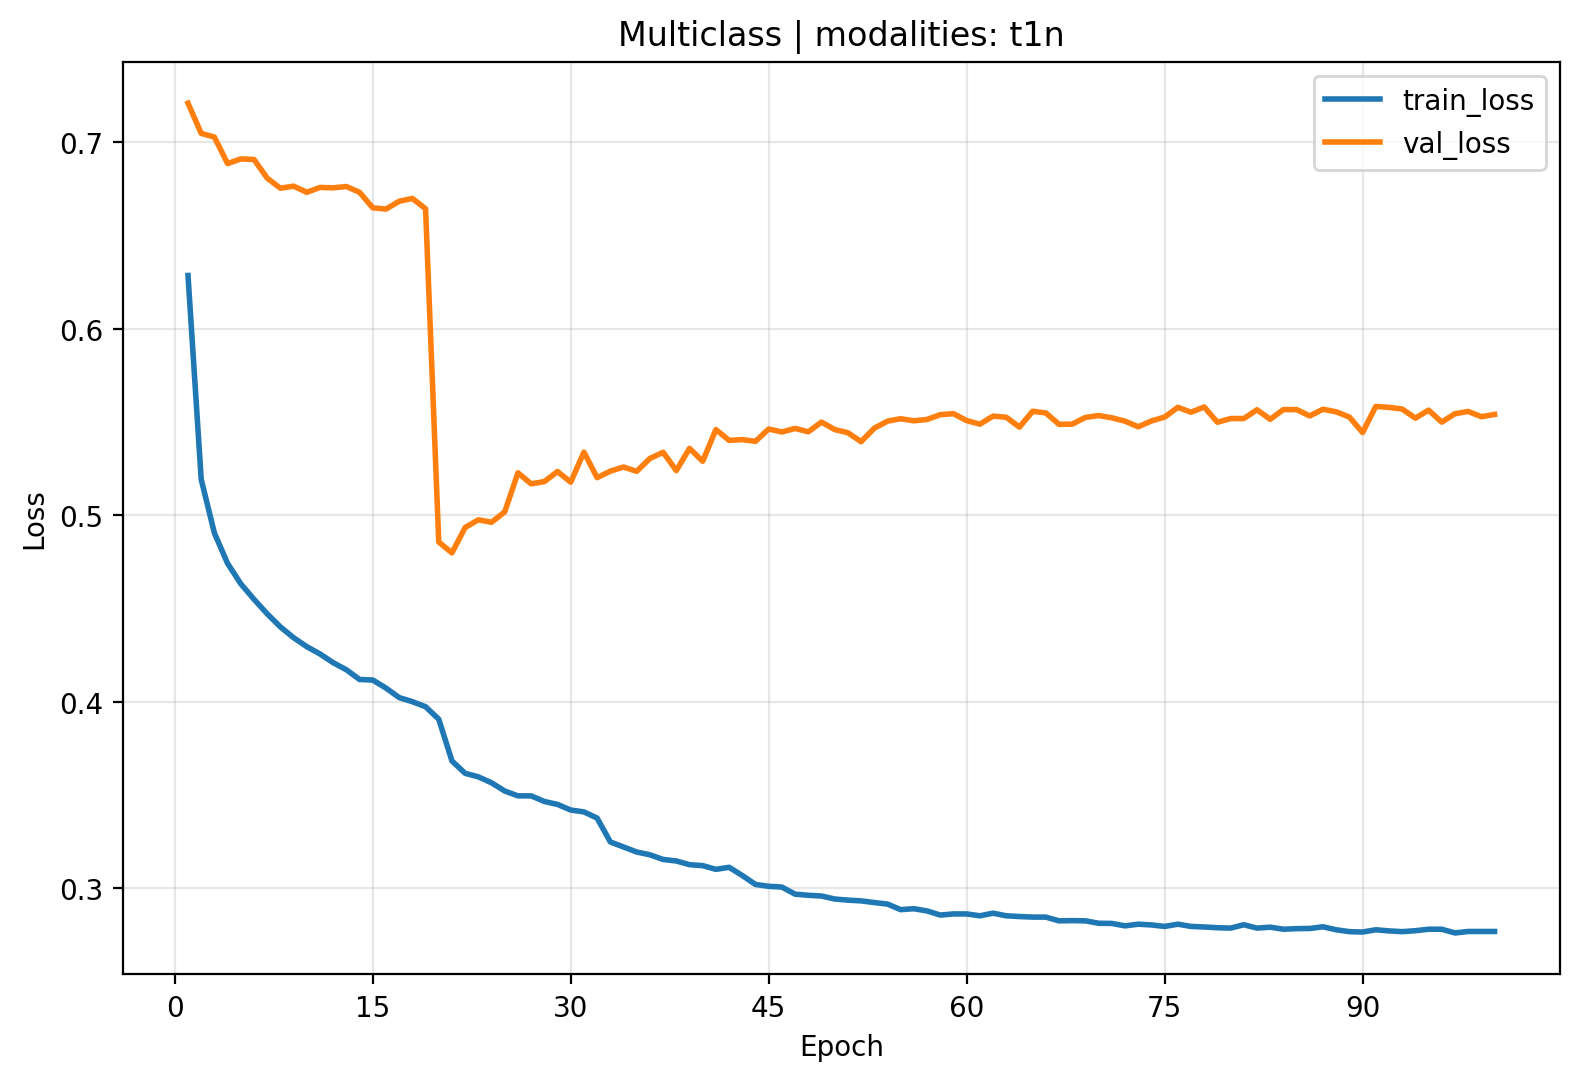
\includegraphics[width=\linewidth,height=0.24\textheight,keepaspectratio]{loss_curve_multiclass_t1n.png}\\[0.3em]
\footnotesize Loss curve for the \texttt{t1n}-only baseline.
\end{minipage}
\hfill
\begin{minipage}[t]{0.45\linewidth}
\centering

\includegraphics[width=\linewidth,height=0.24\textheight,keepaspectratio]{evaluation_outputs/multiclass_t1n/visuals_selected_patients/BraTS-GLI-00022-000_slice_102.png}\\[0.3em]
\footnotesize Representative prediction for BraTS-GLI-00022-000, slice 102.
\end{minipage}
\caption{\texttt{t1n}-only baseline: training curve and representative qualitative result.}
\label{fig:t1nmodel}
\end{figure}

\subsection{\texttt{t1c}-only Multiclass Baseline}

\subsubsection{Purpose}

This baseline uses only \texttt{t1c}. It tests how far contrast-enhanced information alone can support tumor segmentation, especially for TC and ET.

\subsubsection{Quantitative Result}

The mean Dice improves to 0.8525. TC reaches 0.9053 and ET reaches 0.8730, confirming that \texttt{t1c} is much more informative than \texttt{t1n} for core and enhancing tumor. However, WT Dice remains 0.7791, suggesting that \texttt{t1c} alone does not fully capture edema and whole-tumor extent.

\subsubsection{Loss Curve and Visualization}

\begin{figure}[h]
\centering
\begin{minipage}[t]{0.45\linewidth}
\centering
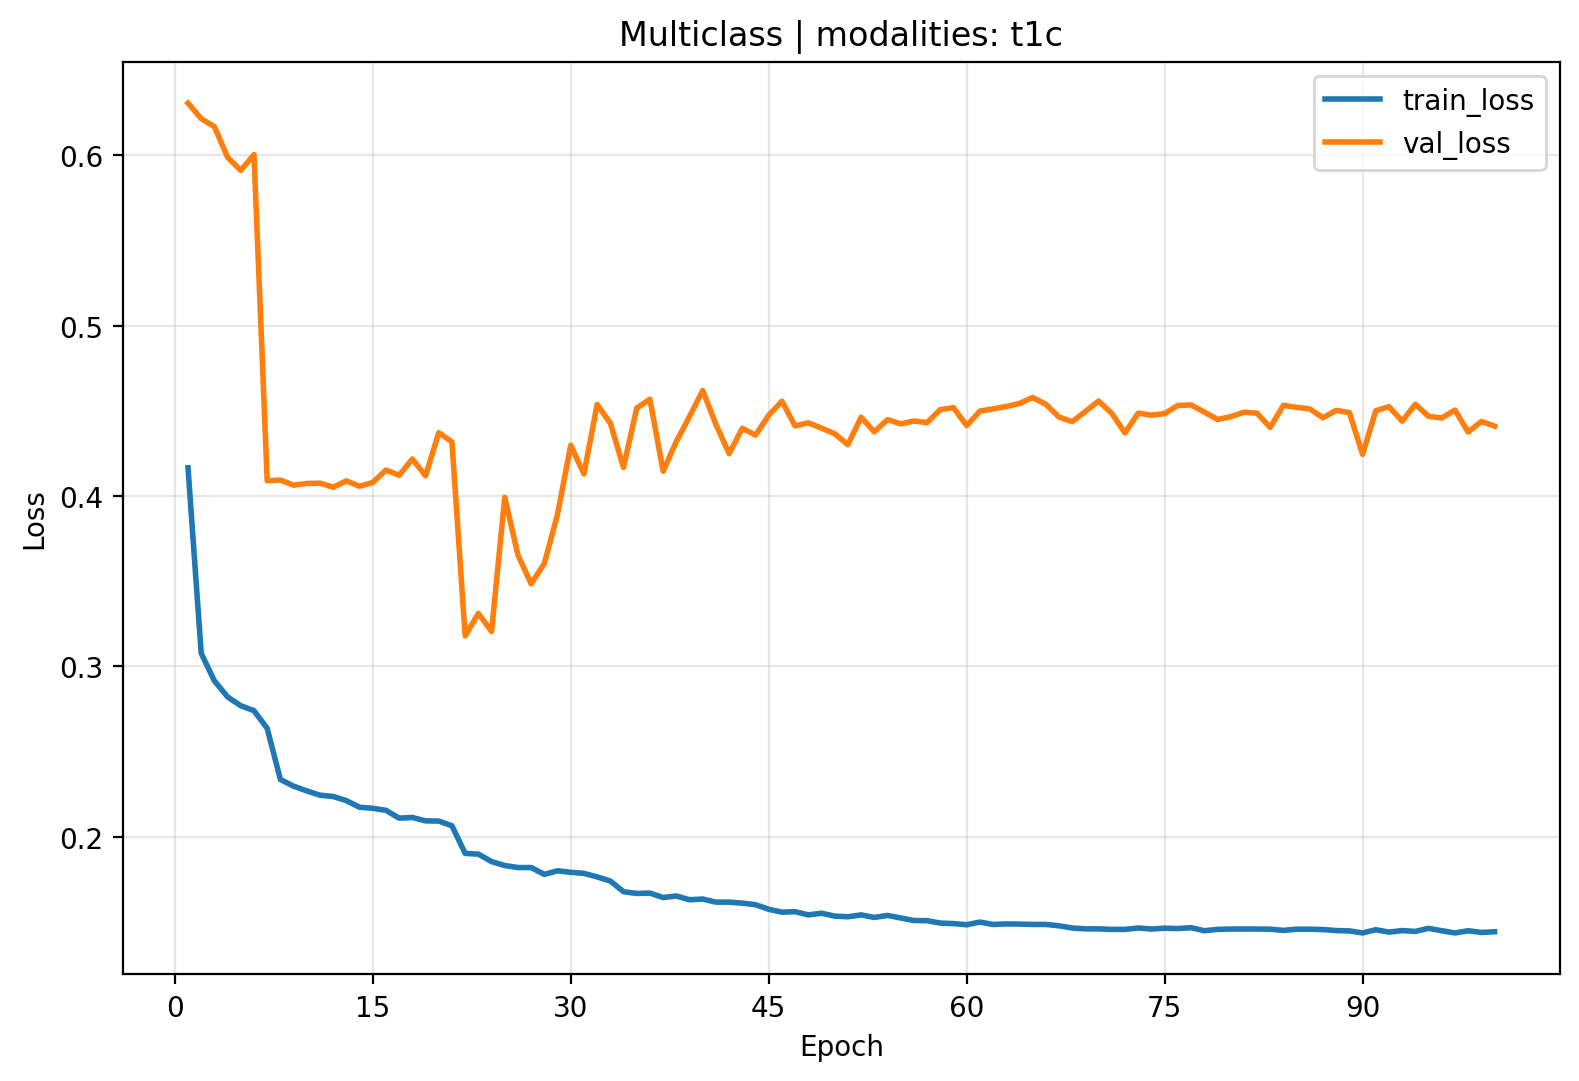
\includegraphics[width=\linewidth,height=0.24\textheight,keepaspectratio]{loss_curve_multiclass_t1c.png}\\[0.3em]
\footnotesize Loss curve for the \texttt{t1c}-only baseline.
\end{minipage}
\hfill
\begin{minipage}[t]{0.45\linewidth}
\centering

\includegraphics[width=\linewidth,height=0.24\textheight,keepaspectratio]{evaluation_outputs/multiclass_t1c/visuals_selected_patients/BraTS-GLI-00022-000_slice_102.png}\\[0.3em]
\footnotesize Representative prediction for BraTS-GLI-00022-000, slice 102.
\end{minipage}
\caption{\texttt{t1c}-only baseline: training curve and representative qualitative result.}
\label{fig:t1cmodel}
\end{figure}

\subsection{Selected Multimodal Input: \texttt{t2f + t1c + t2w}}

\subsubsection{Purpose}

This model tests the main hypothesis that complementary modalities improve segmentation. \texttt{t2f} contributes strong whole-tumor and edema contrast, \texttt{t1c} contributes enhancement and tumor-core information, and \texttt{t2w} adds fluid-sensitive structural support.

\subsubsection{Quantitative Result}

This is the best model in the current experiments. It reaches a mean Dice of 0.9295, with WT = 0.9369, TC = 0.9519, and ET = 0.8997. The improvement over both single-modality baselines shows that the modalities provide complementary information.

\subsubsection{Loss Curve and Visualization}

\begin{figure}[h]
\centering
\begin{minipage}[t]{0.45\linewidth}
\centering
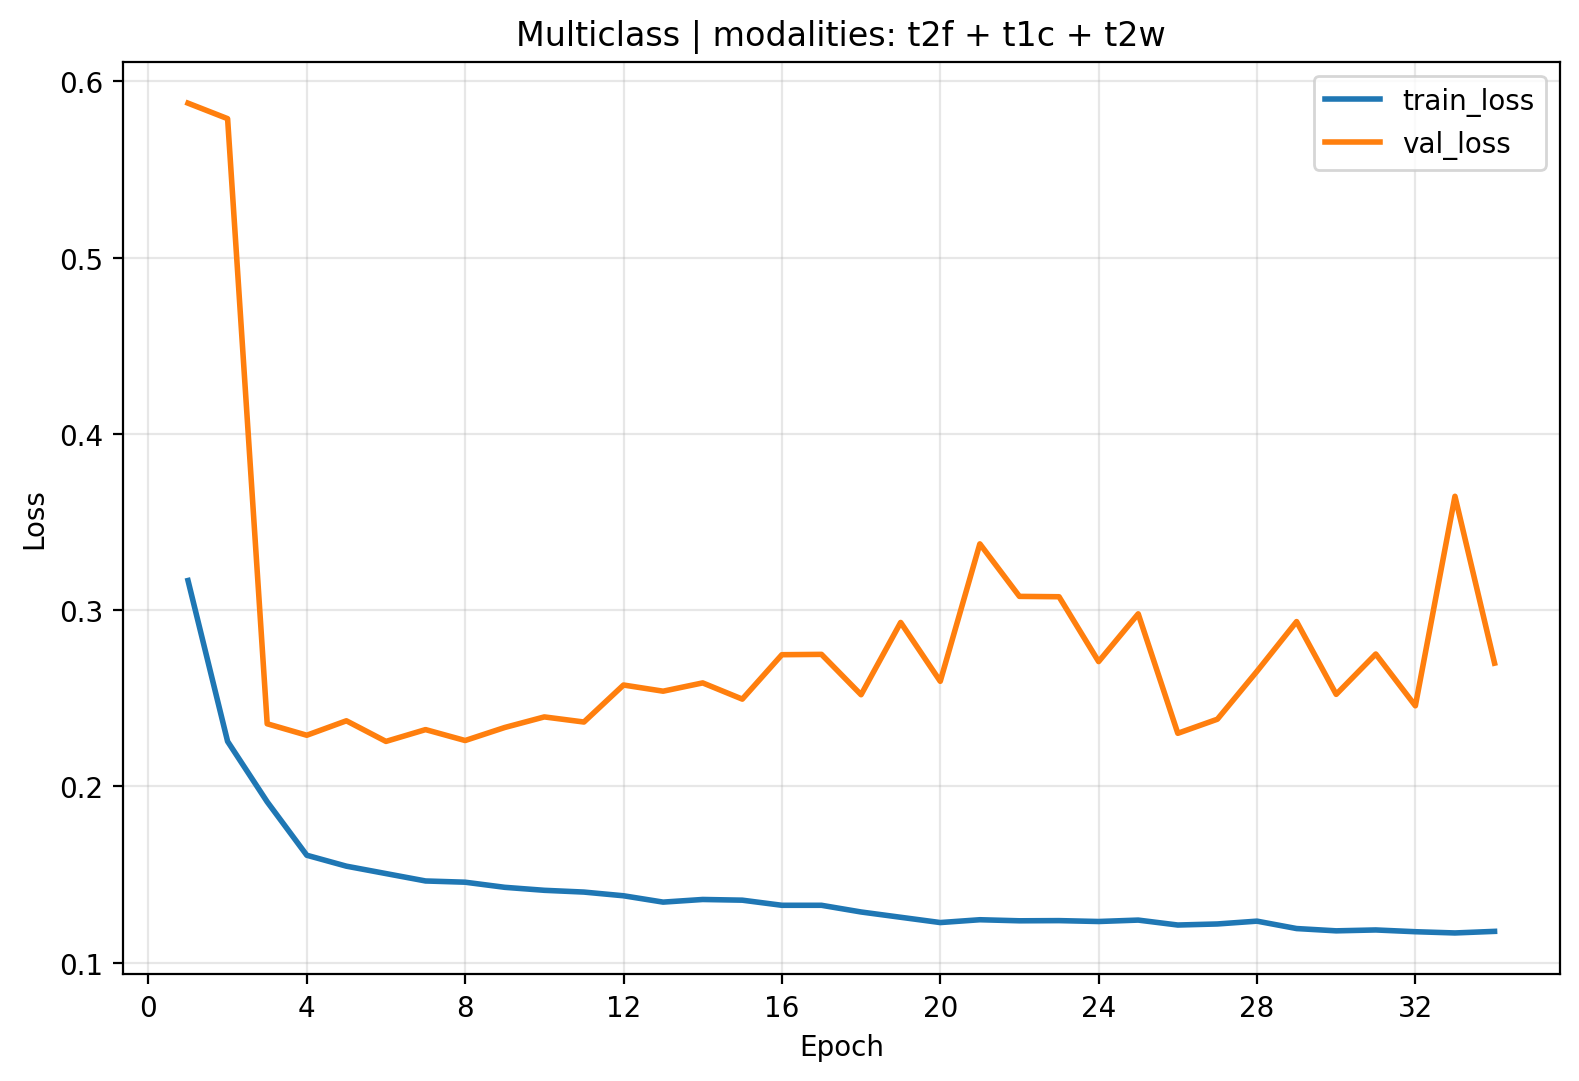
\includegraphics[width=\linewidth,height=0.24\textheight,keepaspectratio]{loss_curve_multiclass_t2f_t1c_t2w.png}\\[0.3em]
\footnotesize Loss curve for the selected three-modality multiclass model.
\end{minipage}
\hfill
\begin{minipage}[t]{0.45\linewidth}
\centering

\includegraphics[width=\linewidth,height=0.24\textheight,keepaspectratio]{evaluation_outputs/multiclass_t2f_t1c_t2w/visuals_selected_patients/BraTS-GLI-00022-000_slice_102.png}\\[0.3em]
\footnotesize Representative prediction for BraTS-GLI-00022-000, slice 102.
\end{minipage}
\caption{Selected three-modality multiclass model: training curve and representative qualitative result.}
\label{fig:selectedmodel}
\end{figure}

\subsubsection{Comparison with Single-Modality Baselines}

\begin{figure}[h]
\centering
\begin{minipage}[t]{0.30\linewidth}
\centering

\includegraphics[width=\linewidth,height=0.20\textheight,keepaspectratio]{evaluation_outputs/multiclass_t1n/visuals_selected_patients/BraTS-GLI-00022-000_slice_102.png}\\[0.3em]
\footnotesize \texttt{t1n}-only
\end{minipage}
\hfill
\begin{minipage}[t]{0.30\linewidth}
\centering

\includegraphics[width=\linewidth,height=0.20\textheight,keepaspectratio]{evaluation_outputs/multiclass_t1c/visuals_selected_patients/BraTS-GLI-00022-000_slice_102.png}\\[0.3em]
\footnotesize \texttt{t1c}-only
\end{minipage}
\hfill
\begin{minipage}[t]{0.30\linewidth}
\centering

\includegraphics[width=\linewidth,height=0.20\textheight,keepaspectratio]{evaluation_outputs/multiclass_t2f_t1c_t2w/visuals_selected_patients/BraTS-GLI-00022-000_slice_102.png}\\[0.3em]
\footnotesize Selected 3 modalities
\end{minipage}
\caption{Qualitative comparison on the same slice: \texttt{t1n}-only, \texttt{t1c}-only, and selected multimodal input.}
\label{fig:modalitycomparison}
\end{figure}

\subsection{All-Modality Input: \texttt{t1n + t1c + t2w + t2f}}

\subsubsection{Purpose}

The all-modality model tests whether using every available MRI sequence automatically improves performance. This is important because more input channels may add useful information, but may also introduce weak or redundant features.

\subsubsection{Quantitative Result}

The all-modality model reaches a mean Dice of 0.9158. This is strong, but still below the selected three-modality model. Therefore, adding \texttt{t1n} does not guarantee better segmentation in this baseline setting.

\subsubsection{Loss Curve and Visualization}

\begin{figure}[h]
\centering
\begin{minipage}[t]{0.45\linewidth}
\centering
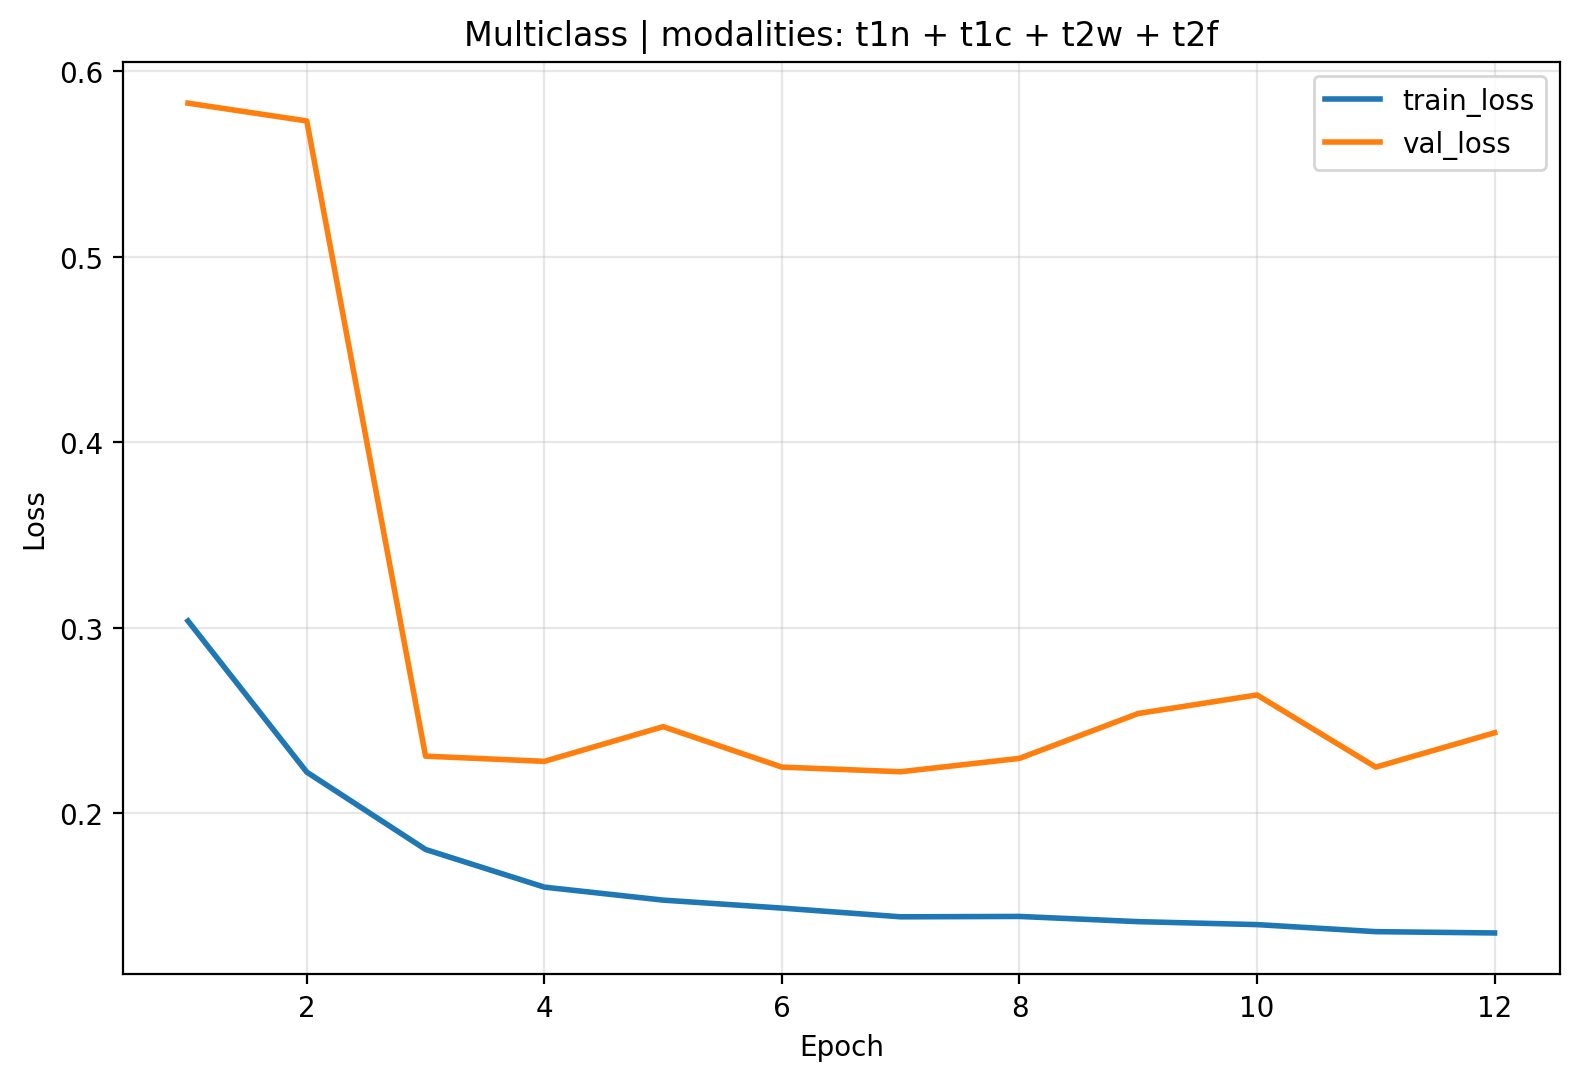
\includegraphics[width=\linewidth,height=0.24\textheight,keepaspectratio]{loss_curve_multiclass_all_modalities.png}\\[0.3em]
\footnotesize Loss curve for the all-modality multiclass model.
\end{minipage}
\hfill
\begin{minipage}[t]{0.45\linewidth}
\centering
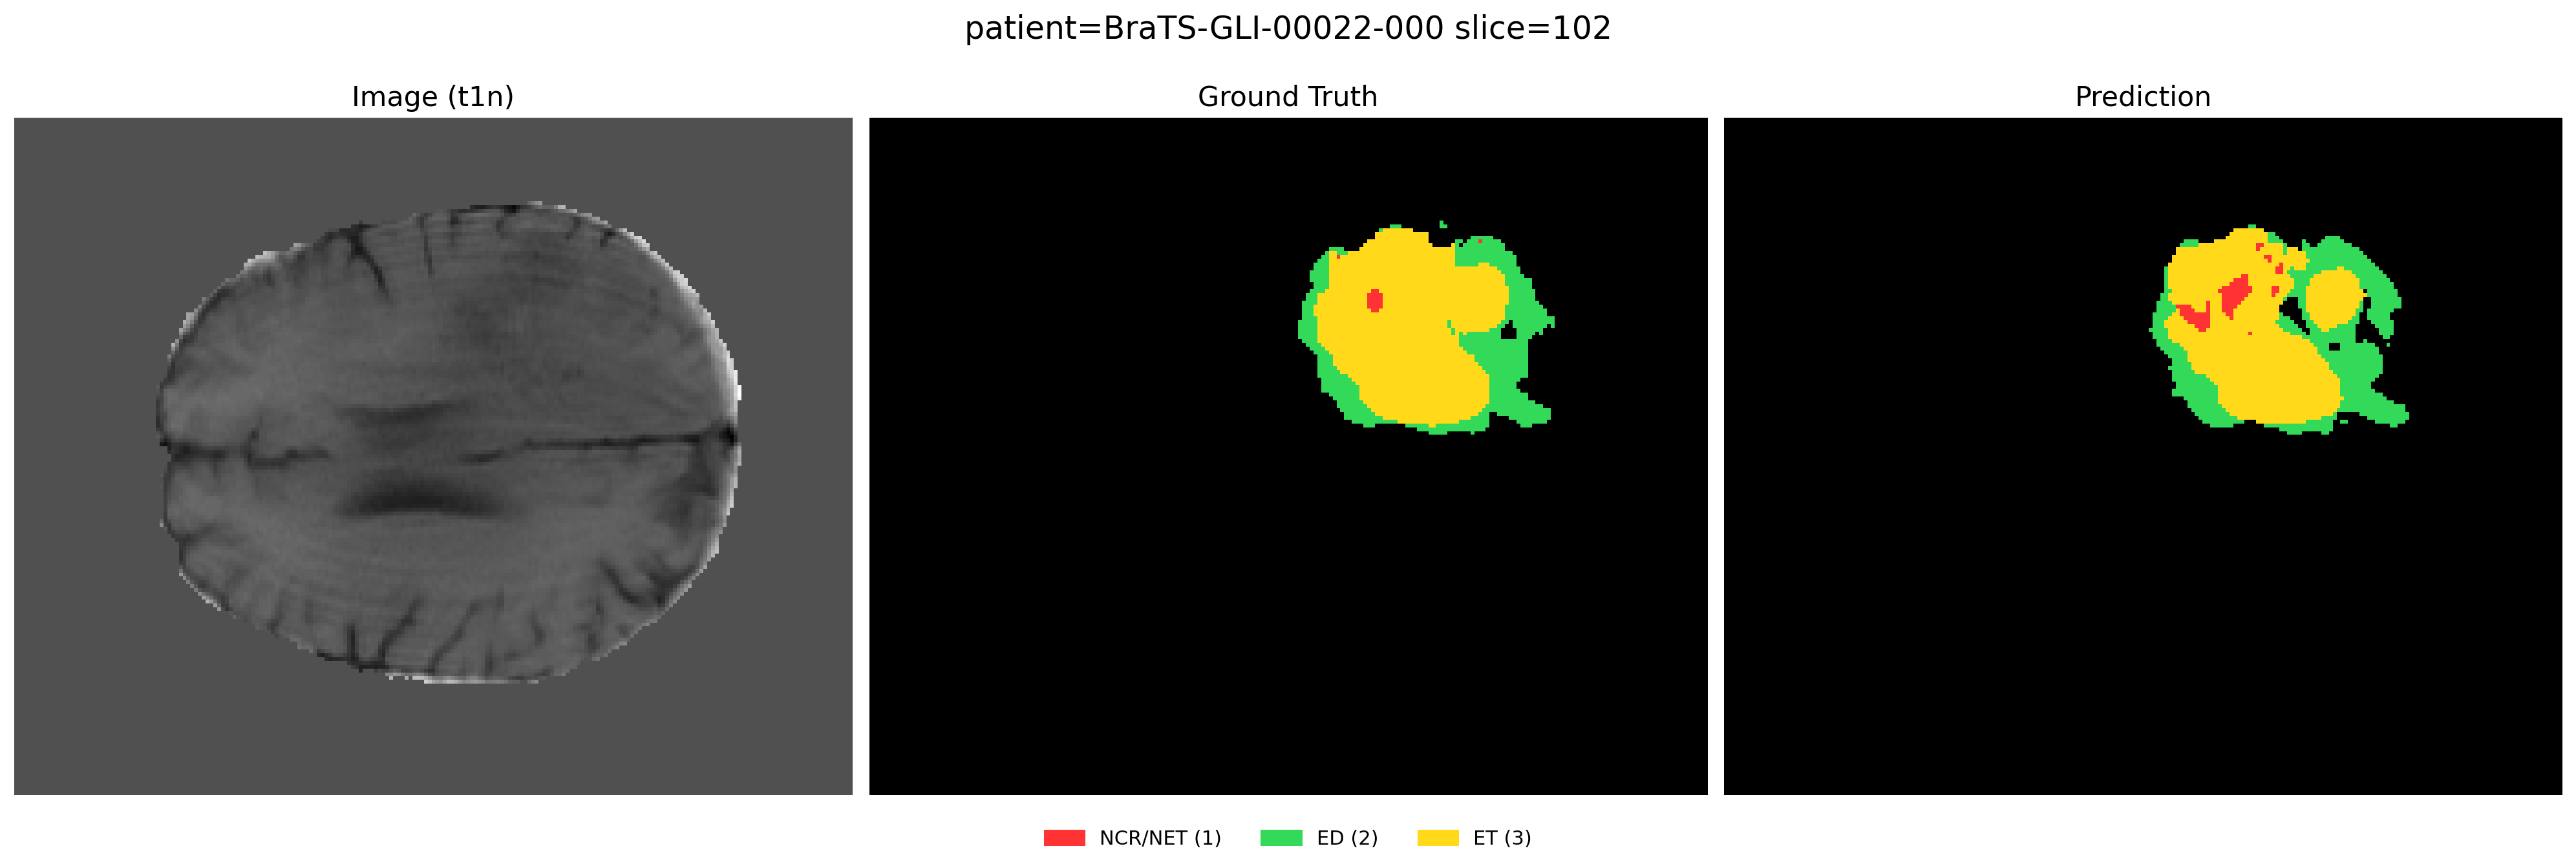
\includegraphics[width=\linewidth,height=0.24\textheight,keepaspectratio]{evaluation_outputs/multiclass_all_modalities/visuals_selected_patients/BraTS-GLI-00022-000_slice_102.png}\\[0.3em]
\footnotesize Representative prediction for BraTS-GLI-00022-000, slice 102.
\end{minipage}
\caption{All-modality multiclass model: training curve and representative qualitative result.}
\label{fig:allmodel}
\end{figure}

\subsection{Region-Based Output Using the Selected Modalities}

\subsubsection{Purpose}

This model uses the selected modalities but predicts WT, TC, and ET directly as three binary maps. The purpose is to test whether direct clinical-region prediction improves Dice scores compared with predicting the original multiclass labels first.

\subsubsection{Quantitative Result}

The region-based model reaches a mean Dice of 0.9074. This is competitive, but lower than the multiclass model with the same modalities. The likely reason is that WT, TC, and ET are nested regions, but independent binary prediction does not automatically enforce this structure.

\subsubsection{Loss Curve and Visualization}

\begin{figure}[h]
\centering
\begin{minipage}[t]{0.45\linewidth}
\centering
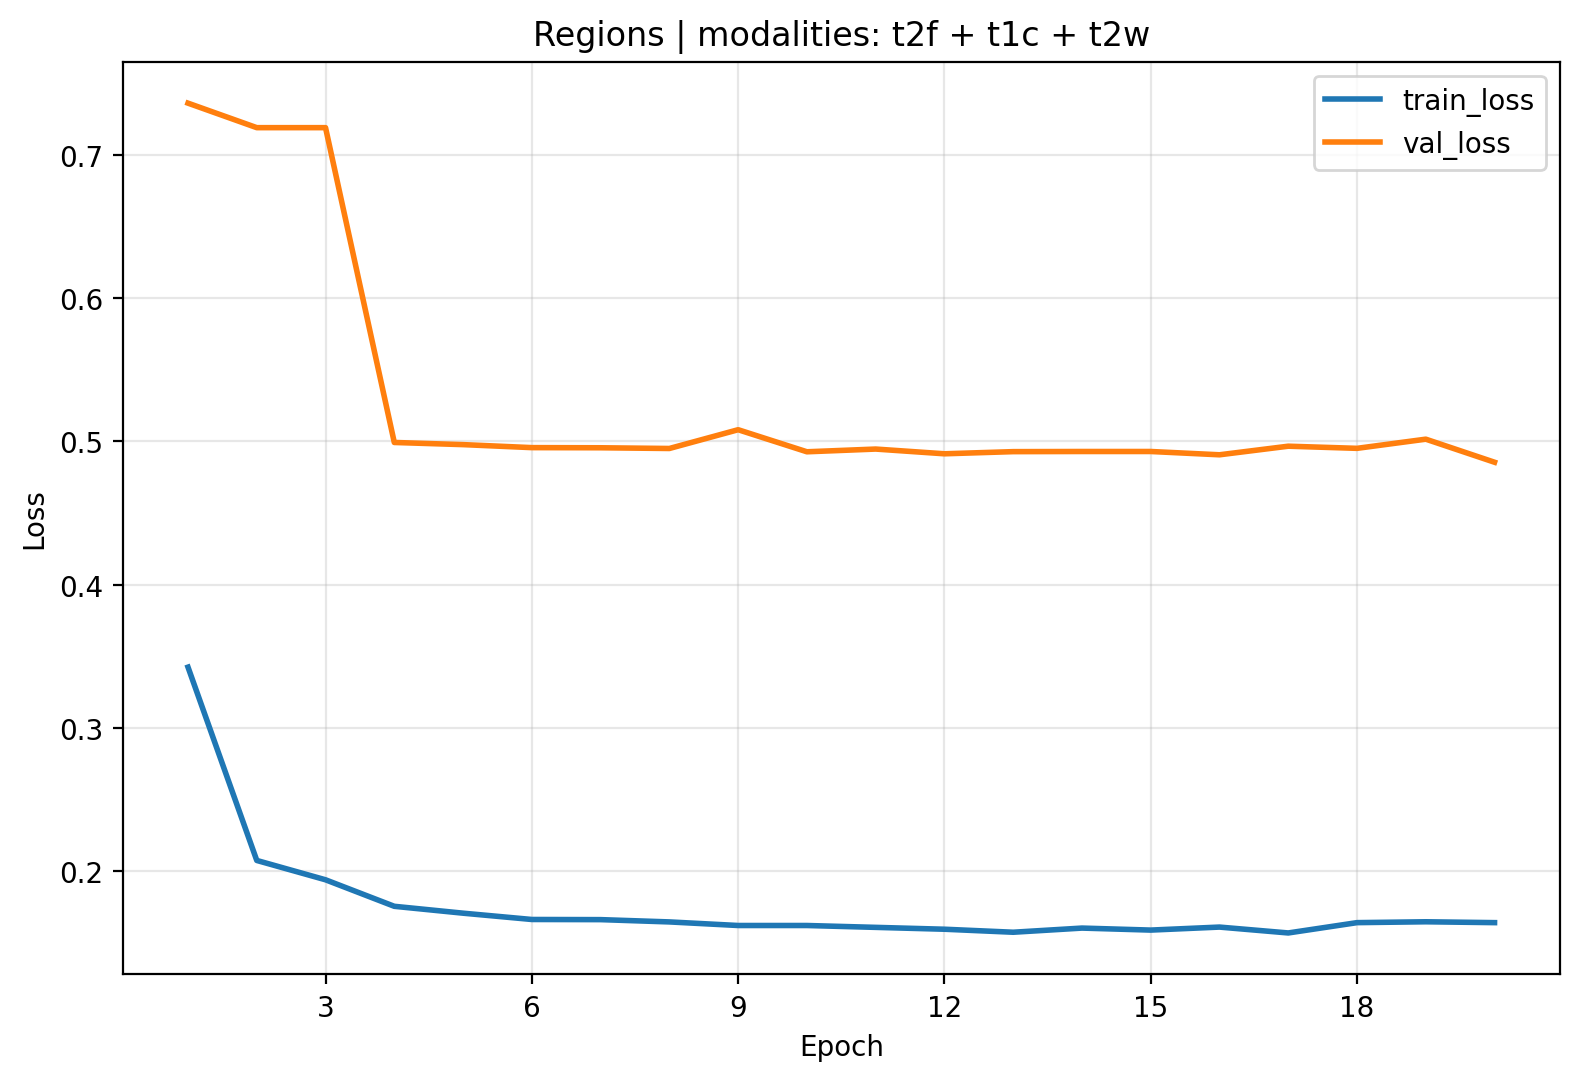
\includegraphics[width=\linewidth,height=0.24\textheight,keepaspectratio]{loss_curve_regions_t2f_t1c_t2w.png}\\[0.3em]
\footnotesize Loss curve for the region-based selected-modality model.
\end{minipage}
\hfill
\begin{minipage}[t]{0.45\linewidth}
\centering

\includegraphics[width=\linewidth,height=0.24\textheight,keepaspectratio]{evaluation_outputs/regions_t2f_t1c_t2w/visuals_selected_patients/BraTS-GLI-00022-000_slice_102.png}\\[0.3em]
\footnotesize Representative prediction for BraTS-GLI-00022-000, slice 102.
\end{minipage}
\caption{Region-based model: training curve and representative qualitative result.}
\label{fig:regionmodel}
\end{figure}

\begin{figure}[h]
\centering
\begin{minipage}[t]{0.43\linewidth}
\centering

\includegraphics[width=\linewidth,height=0.20\textheight,keepaspectratio]{evaluation_outputs/multiclass_t2f_t1c_t2w/visuals_selected_patients/BraTS-GLI-00022-000_slice_102.png}\\[0.3em]
\footnotesize Multiclass output
\end{minipage}
\hfill
\begin{minipage}[t]{0.43\linewidth}
\centering

\includegraphics[width=\linewidth,height=0.20\textheight,keepaspectratio]{evaluation_outputs/regions_t2f_t1c_t2w/visuals_selected_patients/BraTS-GLI-00022-000_slice_102.png}\\[0.3em]
\footnotesize Region output
\end{minipage}
\caption{Qualitative comparison on the same slice between multiclass prediction and direct region prediction.}
\label{fig:targetcomparison}
\end{figure}

This comparison supports the final choice of multiclass prediction. The region-based formulation is clinically intuitive, but for this baseline it introduces additional structural complexity without improving the final Dice score.

\subsection{Conclusion}

This task establishes a complete and reproducible baseline for 2D brain tumor segmentation. The final selected model uses a simple 2D U-Net, Dice + Cross Entropy loss, paired data augmentation, patient-level splitting, and validation-based learning rate decay. The experiments show that both input modality selection and target formulation matter. The selected three-modality input \texttt{t2f + t1c + t2w} performs better than the single-modality baselines and also outperforms the all-modality run in the current Dice results. The multiclass target formulation performs better than the region-based formulation while remaining simpler and more structurally consistent. The final selected model achieves Dice scores of 0.9369 for WT, 0.9519 for TC, and 0.8997 for ET, with a mean Dice of 0.9295.

Overall, the model comparison shows a clear performance trend. The weakest model is the \texttt{t1n}-only baseline, with a mean Dice of 0.6359. This confirms that anatomical T1 information alone is not sufficient for accurate tumor segmentation. The \texttt{t1c}-only model improves substantially to 0.8525 mean Dice, mainly because contrast enhancement provides much stronger information for TC and ET. The selected multimodal input then raises the performance further, showing that edema-sensitive and enhancement-sensitive modalities complement each other. The earlier selected-modality multiclass run reaches 0.9014 mean Dice, while the later selected-modality run reaches the best score of 0.9295.

The all-modality model also performs strongly, with a mean Dice of 0.9158, but it does not exceed the best selected three-modality model. This is an important result because it shows that more modalities are not automatically better. Adding \texttt{t1n} increases the number of input channels, but its weak tumor-background contrast does not necessarily improve the segmentation. Therefore, the selected \texttt{t2f + t1c + t2w} combination is a better balance between information content and input simplicity.

The comparison between multiclass and region-based outputs also supports the final design choice. With the same selected modalities, the region-based model reaches 0.9074 mean Dice, while the multiclass model reaches 0.9295. This suggests that directly predicting WT, TC, and ET is reasonable but not optimal for this baseline. The multiclass formulation benefits from predicting the original mutually exclusive labels first, then deriving WT, TC, and ET for evaluation. As a result, the final selected configuration is the \texttt{t2f + t1c + t2w} multiclass U-Net.
